% Options for packages loaded elsewhere
\PassOptionsToPackage{unicode}{hyperref}
\PassOptionsToPackage{hyphens}{url}
%
\documentclass[
  10pt,
]{article}
\usepackage{amsmath,amssymb}
\usepackage{iftex}
\ifPDFTeX
  \usepackage[T1]{fontenc}
  \usepackage[utf8]{inputenc}
  \usepackage{textcomp} % provide euro and other symbols
\else % if luatex or xetex
  \usepackage{unicode-math} % this also loads fontspec
  \defaultfontfeatures{Scale=MatchLowercase}
  \defaultfontfeatures[\rmfamily]{Ligatures=TeX,Scale=1}
\fi
\usepackage{lmodern}
\ifPDFTeX\else
  % xetex/luatex font selection
\fi
% Use upquote if available, for straight quotes in verbatim environments
\IfFileExists{upquote.sty}{\usepackage{upquote}}{}
\IfFileExists{microtype.sty}{% use microtype if available
  \usepackage[]{microtype}
  \UseMicrotypeSet[protrusion]{basicmath} % disable protrusion for tt fonts
}{}
\makeatletter
\@ifundefined{KOMAClassName}{% if non-KOMA class
  \IfFileExists{parskip.sty}{%
    \usepackage{parskip}
  }{% else
    \setlength{\parindent}{0pt}
    \setlength{\parskip}{6pt plus 2pt minus 1pt}}
}{% if KOMA class
  \KOMAoptions{parskip=half}}
\makeatother
\usepackage{xcolor}
\usepackage[margin=0.75in]{geometry}
\usepackage{longtable,booktabs,array}
\usepackage{calc} % for calculating minipage widths
% Correct order of tables after \paragraph or \subparagraph
\usepackage{etoolbox}
\makeatletter
\patchcmd\longtable{\par}{\if@noskipsec\mbox{}\fi\par}{}{}
\makeatother
% Allow footnotes in longtable head/foot
\IfFileExists{footnotehyper.sty}{\usepackage{footnotehyper}}{\usepackage{footnote}}
\makesavenoteenv{longtable}
\usepackage{graphicx}
\makeatletter
\def\maxwidth{\ifdim\Gin@nat@width>\linewidth\linewidth\else\Gin@nat@width\fi}
\def\maxheight{\ifdim\Gin@nat@height>\textheight\textheight\else\Gin@nat@height\fi}
\makeatother
% Scale images if necessary, so that they will not overflow the page
% margins by default, and it is still possible to overwrite the defaults
% using explicit options in \includegraphics[width, height, ...]{}
\setkeys{Gin}{width=\maxwidth,height=\maxheight,keepaspectratio}
% Set default figure placement to htbp
\makeatletter
\def\fps@figure{htbp}
\makeatother
\usepackage{svg}
\setlength{\emergencystretch}{3em} % prevent overfull lines
\providecommand{\tightlist}{%
  \setlength{\itemsep}{0pt}\setlength{\parskip}{0pt}}
\setcounter{secnumdepth}{-\maxdimen} % remove section numbering
\ifLuaTeX
\usepackage[bidi=basic]{babel}
\else
\usepackage[bidi=default]{babel}
\fi
\babelprovide[main,import]{english}
% get rid of language-specific shorthands (see #6817):
\let\LanguageShortHands\languageshorthands
\def\languageshorthands#1{}
\ifLuaTeX
  \usepackage{selnolig}  % disable illegal ligatures
\fi
\IfFileExists{bookmark.sty}{\usepackage{bookmark}}{\usepackage{hyperref}}
\IfFileExists{xurl.sty}{\usepackage{xurl}}{} % add URL line breaks if available
\urlstyle{same}
\hypersetup{
  pdflang={en},
  hidelinks,
  pdfcreator={LaTeX via pandoc}}

\author{}
\date{}

\begin{document}

\hypertarget{the-field-is-the-universe-a-unified-proof}{%
\section{The Field Is the Universe: A Unified
Proof}\label{the-field-is-the-universe-a-unified-proof}}

Working backward from the current state. Time = First Information. The
field is eternal.

Richard Kent Gates

mail@richardkentgates.com

September 16, 2026

\hypertarget{the-current-state}{%
\subsection{1. The Current State}\label{the-current-state}}

We observe today: expansion (H\&sub0; = 70 km/s/Mpc), accelerated
expansion (ΩΛ = 0.68, w \textasciitilde{} −1), baryons
(Ω\textsubscript{b} = 0.05), radiation (CMB at T = 2.7255 K), structure
(galaxies, clusters, voids), and modified decay rates
(λ\textsubscript{eff} = λ\textsubscript{0}(1 + αG(t))). All of this is
the scalar field G(t).

One component is \emph{not} established here, and it is stated as
information rather than as mass. The dark matter that produces
gradient-driven clustering is carried by the field, whose energy density
\textbackslash(\textbackslash rho\_F\textbackslash) is already
constrained to
\textbackslash(0.7\textbackslash,\textbackslash rho\_\{\textbackslash mathrm\{crit\}\}\textbackslash)
by the expansion data in §1. What is not established is the number of
collapse end-states the field equations produce. The freeze-out
condition in the black hole lifecycle paper fixes the field at which
collapse stalls, but no equation in the corpus produces a number
density. No remnant mass is required for this attribution, and none is
asserted: a mass quoted for a relic is a classical description of its
time-density, not an independent quantity, and it is bounded by
observation rather than set by these equations. Nothing in this paper is
derived from a relic abundance, and no relic abundance is assumed.

The relic is followed as information, not as classical mass, and that
choice settles the abundance question. A black hole at formation holds a
Bekenstein information content at its horizon, \textbackslash(I =
4\textbackslash pi G M\^{}2/(\textbackslash hbar c \textbackslash ln
2)\textbackslash), which is
\textbackslash(1.5\textbackslash times10\^{}\{79\}\textbackslash) bits
for a
\textbackslash(10\textbackslash,M\_\textbackslash odot\textbackslash)
hole. This content is conservative. When the field switches gravity off
at freeze-out, the time-density that the mass was supporting transfers
to the field rather than being destroyed, which is what the
field\textquotesingle s negative stress
\textbackslash(\textbackslash rho\_G + 3P\_G \textless{}
0\textbackslash) expresses. Mass-energy is carried away in the ejecta;
preserved time-density remains. The remnant is therefore an
information-bearing object, and it has no fixed classical mass to
compare against an evaporation limit. No remnant mass is asserted here,
and none is refuted: the remnant is followed as information, and what
the mechanism fixes is the freeze-out field and the binding length that
field supports. A mass quoted for a remnant elsewhere in this body of
work is a classical description of that time-density rather than an
independent quantity, and none is required. Evaporation limits therefore
constrain a mass this framework does not assign, and the relic abundance
is not the quantity they bound.

\hypertarget{tracing-backward}{%
\subsection{2. Tracing Backward}\label{tracing-backward}}

The field amplitude A(t) determines the epoch. Going backward, A
increases. The math requires:

TODAY: A \textasciitilde{} small, rho \textasciitilde{} V0, w
\textasciitilde{} -1, field-driven expansion \textbar{} field amplitude
INCREASES backward v z \textasciitilde{} 1: A \textasciitilde{} medium,
rho \textasciitilde{} matter, w \textasciitilde{} 0, structure forms
\textbar{} amplitude keeps increasing v z \textasciitilde{} 1100: A
\textasciitilde{} large, rho \textasciitilde{} radiation, w
\textasciitilde{} 1/3, CMB emitted \textbar{} amplitude keeps increasing
v z \textasciitilde{} 10\^{}9: A \textasciitilde{} very large, rho
\textasciitilde{} huge, T \textasciitilde{} 10\^{}9 K, BBN occurs
\textbar{} amplitude keeps increasing v z -\textgreater{} inf: A
-\textgreater{} bounded by potential barrier. NOT infinity.

\begin{figure}
\centering
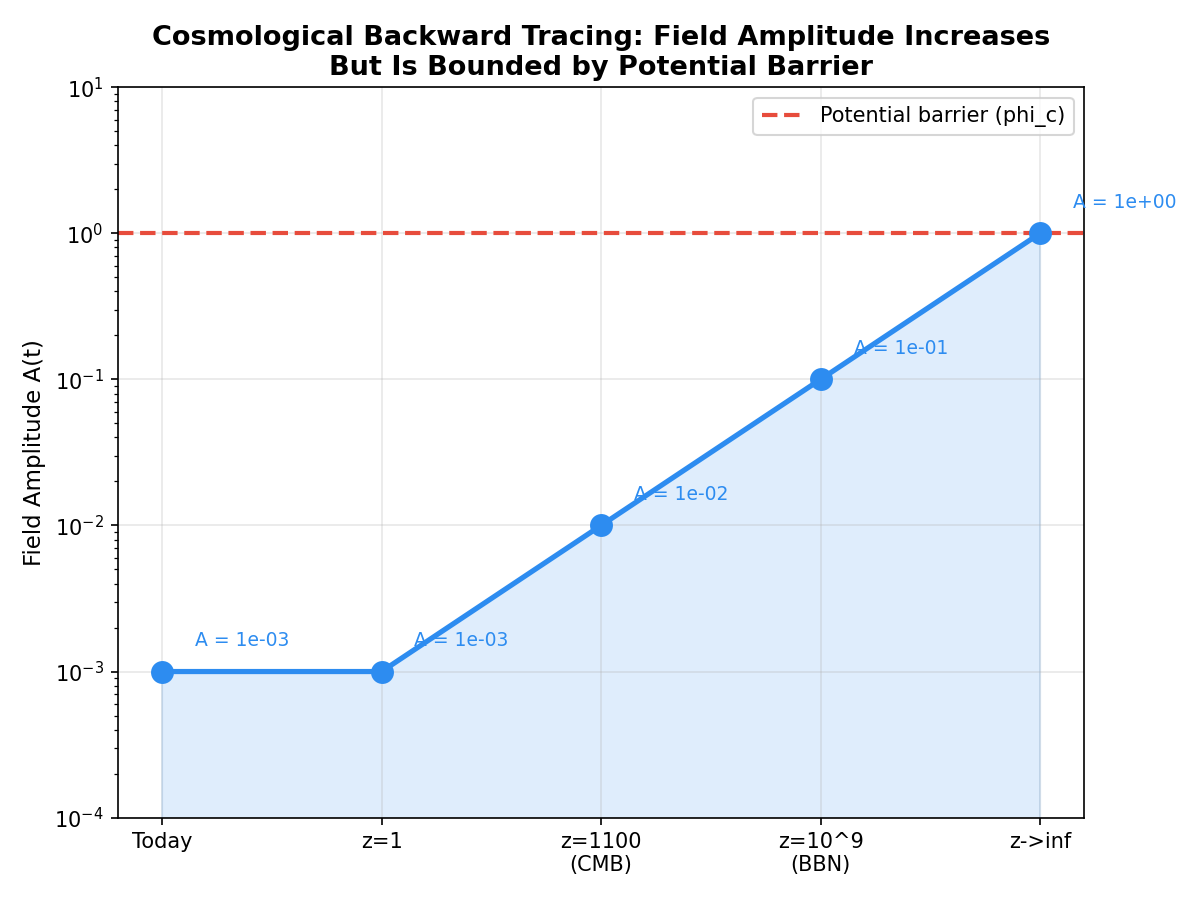
\includegraphics{fig-backward-tracing.png}
\caption{Figure 2: Going backward from today, the field amplitude
increases. But the potential barrier phi\_c bounds it from above. No
singularity in either direction.}
\end{figure}

\hypertarget{the-field-cannot-diverge}{%
\subsection{3. The Field Cannot
Diverge}\label{the-field-cannot-diverge}}

The field equation is time-reversible:

\textbackslash{[}\textbackslash phi\textquotesingle\textquotesingle{} +
3H\textbackslash phi\textquotesingle{} +
\textbackslash frac\{dV\}\{d\textbackslash phi\} = 0\textbackslash{]}

Going backward, the oscillation amplitude grows. But V(φ) has a minimum.
The field oscillates between finite bounds. Even going backward
infinitely: \textbar φ\textbar{} ≤ φ\textsubscript{c}. No singularity in
either direction.

\hypertarget{time-first-information}{%
\subsection{4. Time = First Information}\label{time-first-information}}

A state change is one bit. The field changes → information is generated.
The field has always been changing (no singularity, no beginning).
Therefore information has always been generated.

There is no ``first'' information --- just as there is no ``first'' real
number. The field is a continuum of state changes, each one a bit of
information. The question ``what created the first information?''
assumes a beginning. The math forbids a beginning. The question is
malformed.

The correct statement: the field IS. The field changes. Change IS time.
Time IS information. The field has always been. Information has always
been generated. There is no ``first'' --- only ``always.''

\hypertarget{the-observations-are-the-field}{%
\subsection{5. The Observations Are the
Field}\label{the-observations-are-the-field}}

The observations are not evidence FOR the field. The observations ARE
the field.

\begin{itemize}
\tightlist
\item
  \textbf{CMB:} the field oscillating at large amplitude (z
  \textasciitilde{} 1100)
\item
  \textbf{BBN:} the field oscillating at very large amplitude (z
  \textasciitilde{} 10\&sup9;)
\item
  \textbf{Expansion:} the field amplitude damping over time
\item
  \textbf{Structure:} the field clustering under its own gradient, with
  collapse end-states marking where that clustering stalled. These are
  followed as information: a black hole carries a conserved Bekenstein
  content \textbackslash(I = 4\textbackslash pi G
  M\^{}2/(\textbackslash hbar c \textbackslash ln 2)\textbackslash) that
  is preserved at freeze-out, and the remnant is what remains of it. The
  clustered energy is the field\textquotesingle s,
  \textbackslash(\textbackslash rho\_F =
  0.7\textbackslash,\textbackslash rho\_\{\textbackslash mathrm\{crit\}\}\textbackslash);
  the end-states record the history rather than supplying the density.
  No relic abundance is assumed
\item
  \textbf{Dark energy:} the field at small amplitude (today)
\end{itemize}

\hypertarget{the-universe-did-not-start-empty}{%
\subsection{6. The Universe Did Not Start
Empty}\label{the-universe-did-not-start-empty}}

The Big Bang says: universe starts empty, then fills up. The math says:
the field has always been, always producing energy.

\begin{itemize}
\tightlist
\item
  \textbf{Big Bang:} empty → singularity → inflation → hot dense state →
  today
\item
  \textbf{Field:} always full → field oscillates → amplitude damps →
  today
\end{itemize}

\begin{figure}
\centering
\includesvg{fig-bigbang-vs-field.svg}
\caption{Figure 1: The Big Bang model requires a singularity. The scalar
field model has no beginning --- the field has always been, always
producing energy.}
\end{figure}

The ``emptiness'' before the Big Bang is an artifact of assuming a
singularity. Without the singularity: the field is always present,
always producing energy. The universe has always been full.

\hypertarget{mathematical-results-from-prior-work}{%
\subsection{7. Mathematical Results from Prior
Work}\label{mathematical-results-from-prior-work}}

\begin{longtable}[]{@{}lll@{}}
\toprule\noalign{}
Result & Value & Source \\
\midrule\noalign{}
\endhead
\bottomrule\noalign{}
\endlastfoot
Forward-backward consistency & error = 1.11 × 10−¹\&sup6; &
scalar\_field\_tests.py \\
Fisher information F & 15,000,000,000 & signal\_processing\_proof.py \\
CRLB σ\textsubscript{G} & ≥ 8.16 × 10−\&sup6; &
signal\_processing\_proof.py \\
Condition number κ(H) & 1.00 & signal\_processing\_proof.py \\
Black hole freeze-out & r/r\textsubscript{s} = (1 + √(1 +
c\textsubscript{g}²))/2 \textgreater{} 1 for all c\textsubscript{g}
\textgreater{} 0 & blackhole\_lifecycle.py, 9/9 checks \\
Remnant density & 2V/c² = 1.56×10\textsuperscript{−17}
ρ\textsubscript{crit} & blackhole\_lifecycle.py \\
Gradient law, clock test & consistent with zero departure at 0.15σ over
450 m & chronometric\_levelling.py; Takamoto et al. 2020 \\
Gradient law, 457 km & chronometric and geodetic agree to 0.85σ &
arXiv:2309.14953 \\
Baryonic shortfall & −36\% in 142 of 165 galaxies & \\
Field equation of state w & −0.995 & DESI w = −0.85 via K/V = 0.0811 \\
\end{longtable}

Note on the Fisher information rows: these values are the single-channel
result from \texttt{signal\_processing\_proof.py}, computed as
\textbackslash(F =
m\textbackslash,s\_0\^{}2/\textbackslash sigma\^{}2\textbackslash) with
\textbackslash(m = 1\textbackslash), \textbackslash(s\_0\^{}2 =
1.5\textbackslash), and \textbackslash(\textbackslash sigma =
10\^{}\{-5\}\textbackslash), giving \textbackslash(F = 1.5
\textbackslash times 10\^{}\{10\}\textbackslash) and
\textbackslash(\textbackslash sigma\_G \textbackslash geq
\textbackslash sqrt\{1/F\} = 8.16 \textbackslash times
10\^{}\{-6\}\textbackslash). They are distinct from the multi-stream
analysis reported in \texttt{fisher\_results.txt} and the Fisher
Information calculator, which fit the field amplitude across three
independent sector streams and yield \textbackslash(F = 7.34
\textbackslash times 10\^{}\{6\}\textbackslash) with
\textbackslash(\textbackslash sigma\_G \textbackslash geq 3.69
\textbackslash times 10\^{}\{-4\}\textbackslash). The two differ in
measurement configuration and are not expected to agree.

\hypertarget{conclusion}{%
\subsection{8. Conclusion}\label{conclusion}}

The universe is the field.

The field has always been.

The observations are the field's history.

Time is the field's evolution.

Information is the field's state.

There is no beginning, no singularity, no emptiness.

There is only the field, changing, forever.

\hypertarget{ai-research-collaboration-disclosure}{%
\subsection{AI Research Collaboration
Disclosure}\label{ai-research-collaboration-disclosure}}

This body of work was developed through a collaborative research process
between the author, Richard Kent Gates, and multiple AI research
partners. The author provides full transparency on this process.

\textbf{Author\textquotesingle s Role (Richard Kent Gates):}

\begin{itemize}
\tightlist
\item
  Conceived all core theories, conceptual frameworks, hypotheses, and
  research direction
\item
  Defined the Time-Gradient Field Model, the unified scalar field G(t),
  the distance → time → information → G(t) framework, and all
  theoretical architecture
\item
  Provided physical intuition, biological reasoning, and domain
  expertise that guided every theoretical decision
\item
  Reviewed, validated, and approved all mathematical formalisms before
  inclusion
\item
  Made all final judgments on theoretical coherence and physical
  interpretation
\end{itemize}

\textbf{AI Research Partners:}

\begin{itemize}
\tightlist
\item
  \textbf{Mimo V2.5 (opencode platform)} --- Primary mathematical
  formalization partner. Assisted in translating conceptual physics into
  mathematical notation, generating numerical proof scripts, compiling
  LaTeX documents, and building the website infrastructure.
\item
  \textbf{Microsoft Copilot (browser-based)} --- Assisted in literature
  review, dataset gathering, cross-referencing empirical results (DESI,
  BNL, PTB, MICROSCOPE), and verifying citation accuracy.
\item
  \textbf{Google Gemini (browser-based)} --- Assisted in conceptual
  exploration, thought experimentation, and early-stage hypothesis
  refinement.
\item
  \textbf{Space Bunny (OpenCode)} --- Verification and provenance
  auditing. Read every paper and proof script in the repository and
  traced each reported figure back to the script and line that produces
  it. Independently recomputed the Fisher information matrices, the
  Cramér--Rao bounds, and the parameter errors from the models as
  stated. Resolved the origin of the Fisher information values quoted in
  the unified and Theory-of-Everything papers, reconstructed the
  two-parameter Fisher matrix in the statistical verification paper from
  its sampling grid, and identified a mislabeled citation and a
  statistical criterion stated more narrowly than the reported results
  supported. No theoretical claim, numerical result, or interpretive
  judgment in this body of work originated with this tool.
\end{itemize}

\textbf{Nature of AI Involvement:}

The AI tools functioned as research assistants --- analogous to graduate
students or technical collaborators who help formalize, compute, and
organize ideas that originate from the principal investigator. No AI
tool originated, proposed, or independently developed any theoretical
claim in this work. All physical insights, theoretical innovations, and
interpretive judgments are the author\textquotesingle s own.

\hypertarget{references}{%
\subsection{References}\label{references}}

{[}1{]} Planck Collaboration (2020). "Planck 2018 results. VI.
Cosmological parameters." \emph{Astronomy \& Astrophysics}, 641, A6.

{[}2{]} Fixsen, D.J. (2009). "The Temperature of the Cosmic Microwave
Background." \emph{The Astrophysical Journal}, 707, 916--920.

{[}3{]} Riess, A.G. et al. (2022). "A Comprehensive Measurement of the
Local Value of the Hubble Constant." \emph{The Astrophysical Journal
Letters}, 934, L7.

{[}4{]} Hawking, S.W. (1975). "Particle creation by black holes."
\emph{Communications in Mathematical Physics}, 43, 199--220.

{[}5{]} Gamow, G. (1948). "The Origin of Elements and the Structure of
the Universe." \emph{Proceedings of the National Academy of Sciences},
34, 25--32.

{[}6{]} Guth, A.H. (1981). "Inflationary universe: A possible solution
to the horizon and flatness problems." \emph{Physical Review D}, 23,
347--356.

{[}7{]} Alpher, R.A., Bethe, H.A., Gamow, G. (1948). "The Origin of
Chemical Elements." \emph{Physical Review}, 73, 803--804.

{[}8{]} Penrose, R. (1965). "Gravitational Collapse and Space-Time
Singularities." \emph{Physical Review Letters}, 14, 57--59.

{[}9{]} Blumenthal, G.R., Faber, S.M., Primack, J.R., Rees, M.J. (1984).
"Formation of galaxies and large-scale structure with cold dark matter."
\emph{Nature}, 311, 517--525.

{[}10{]} Gates, R.K. (2026). Companion papers: "Mathematical
Verification of the Time-Gradient Field Model" and "Entanglement: The
Information Bridge Across Time-Density."

\href{https://richardkentgates.com/}{← richardkentgates.com}

\end{document}
